 
\section{Appendix 1}
\label{App1}
\section{Transformaci\'on de Coordenadas}
[Montenbruck, Vallado Revisitin, Vallado Coorde Sys, tabla de Boado]

Para la comparaci\'on de las posiciones en coordenadas cartesianas, es necesario llevar ambos vectores a un mismo sistema de referencia.
La figura (ref) muestra un resumen de los distintos sistemas y las consideraciones de cada uno. 

\begin{figure}[!h]
  \centering
  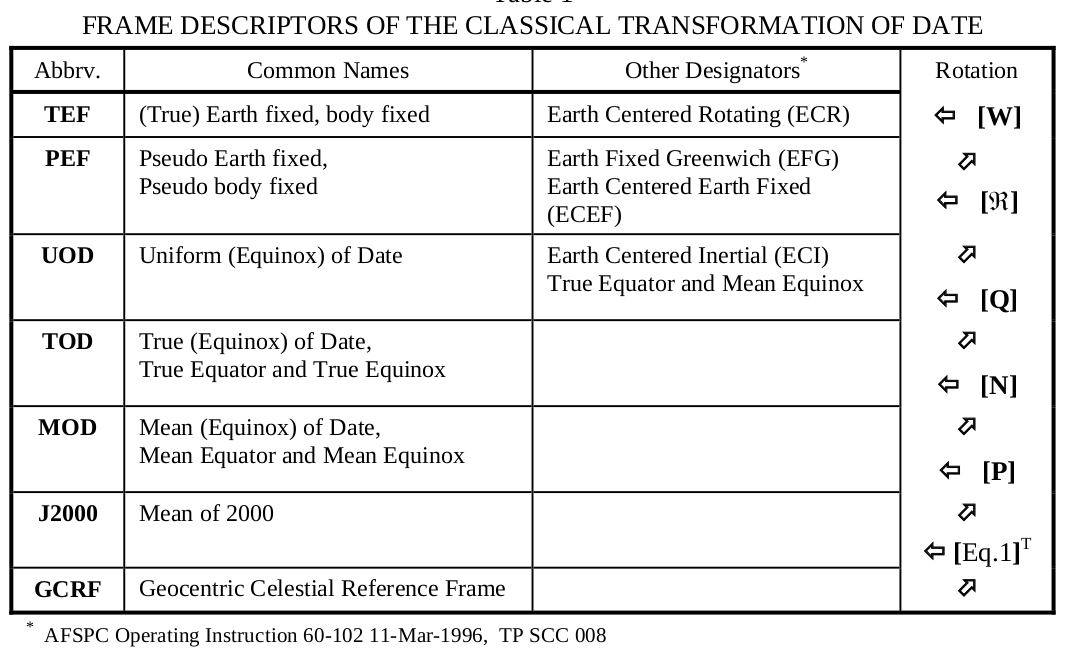
\includegraphics[width=0.7\textwidth]{imagenes/sistReferencias}
\end{figure}

En nuestro caso en particular, los datos que provee CODS se publican en el sistema TOD: True of Date (Verdadero de la \'epoca), mientras que los vectores de estado que genera el propagador SGP4 est\'an calculados en el sistema TEME: True Equator Mean Equinox (Ecuador Verdadero y Equinoccio Medio), tambi\'en denominado UOD (Uniform Equinox of Date).

Para la transformaci\'on de los datos de salida del SGP4 en el sistema TEME, al sistema TOD utilizamos la ecuaci\'on de los equinoccios, $EQ_{equinox}$, que nos permite transformar el equinoccio medio en el equinoccio verdadero.\\
Dado el vector de estado en el sistema TEME, $r_{_{TEME}}$, lo multiplicamos por la matriz de transformaci\'on en el eje z $Rot_{3}(EQ_{equinox})$ y obtenemos el vector de estado en el sistema TOD, $r_{_{TOD}}$.

\begin{equation}
 r_{_{TOD}} = [Q] r_{_{TEME}}
\end{equation}


 \[ Q =
\left( \begin{array}{ccc}
 cos(-EQ_{eqe}) & sin(-EQ_{eqe}) &  0 \\ 
 -sin(-EQ_{eqe}) & cos(-EQ_{eqe}) &  0 \\
 0 & 0 & 1
\end{array} \right) \] 


La ecuaci\'on de los equinoccios utiliza el modelo de nutaci\'on IAU-80 que considera los par\'ametros de nutaci\'on y los 106 coeficientes de Delaunay para el c\'alculo de la longitud $\Delta \Psi$ y la oblicuidad $\Delta \epsilon$.

\begin{equation}
 EQ_{eqe}=\Delta \Psi cos({\epsilon}) + 0.00264 \textquotedbl sin(\Omega_{(}) + 0.000063 \textquotedbl sin (2 \Omega_{(})
\end{equation}

Donde:

\begin{align*}
 \epsilon &= {\bar{\epsilon}} + \Delta \epsilon\\
 \Delta \Psi &= (A_{p} + A_{pl} tt) sin(a_{p_{i}})\\
 \Delta \epsilon &= (A_{e} + A_{el} tt) cos(a_{p_{i}})
\end{align*}

\begin{align*}
 tt &= (jd - 51544.5)/36525.0\\
 {\bar{\epsilon}} &= 84381.448 \textquotedbl - 46.8150 \textquotedbl tt - 0.00059 \textquotedbl tt^{2} + 0.001813 tt^{3}\\
 a_{p_{i}} &= a_{n1}M_{(}+a_{n2}M_{o}+a_{n3}\mu_{(}+a_{n4}D_{o}+a_{n5}\Omega_{(}
\end{align*}

Los coeficientes: $A_{p}$,$A_{pl}$,$A_{e}$,$A_{el}$,$A_{n_{i}}$ se extraen de la tabla de coeficientes de nutaci\'on de Seidelman(citar).

Y el resto de los par\'ametros se calcula seg\'un las expresiones:\\

\begin{align*}
 M_{(} & = M(tt)\\
 M_{o} & = M(tt)\\
 \mu_{(} &= \mu(tt)\\
 D_{o} &= D(tt)\\
 \Omega_{(} &= \Omega(tt)
\end{align*}

%%%%%%%%%%%%%%%%%%%%%%%%%%%%%%%%
\section{Appendix 2}
\label{App2}
